\section{Implementation}
\label{sec:implementation}

This chapter discusses the implementation of the design that was discussed in \autoref{sec:design-and-system-architecture}, and the problems and changes that were encountered during the implementation process.

\subsection{Mechanical Design}
\label{sec:mechanical-design}
As discussed in \autoref{sec:design-and-system-architecture}, the system is designed in FreeCAD \cite{freecad}, a parametric 3D modelling software. The below figures show the system in its entirety, with the front and back views of the system.

\begin{figure}[H]
    \begin{minipage}[h]{0.95\textwidth}
        \centering
        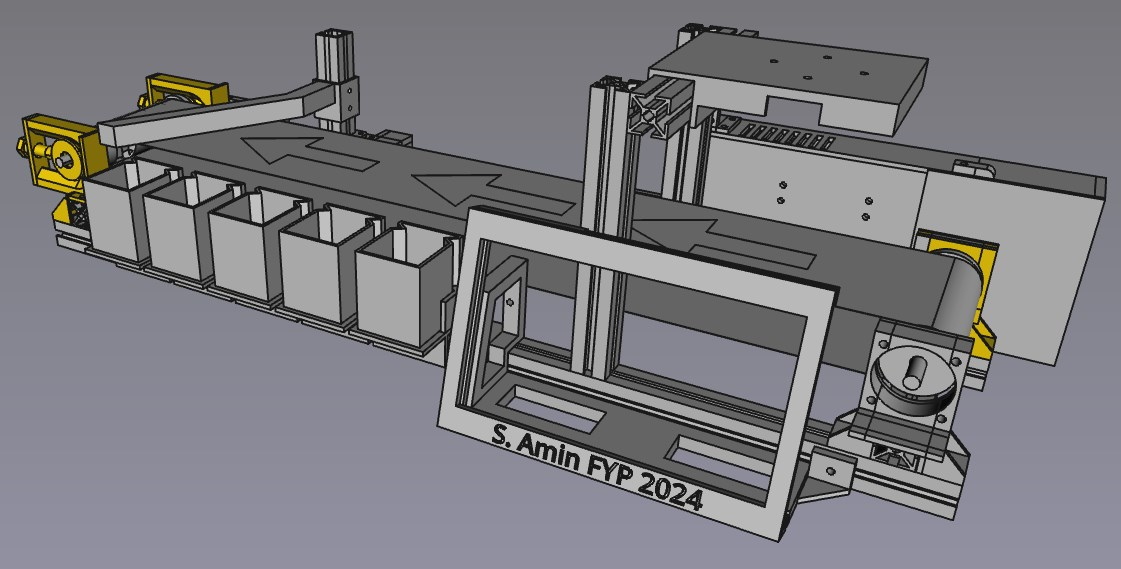
\includegraphics[height=8cm]{imgs/freecad/wholefront.jpg}
        \caption{Front View of the Mechanical Design}
    \end{minipage}
\end{figure}

The conveyor belt with the direction of travel is indicated with arrows. The camera is mounted on the top of the system, with LED lights inside the camera mount. The LCD mount for the DFRobot 7" LCD is clearly visible at the front, with a NEMA17 stepper motor mount positioned next to it for the driven conveyor rollers. The sorting bins are clearly present in the front of the system for easy user access.

\begin{figure}[H]
    \begin{minipage}[h]{0.95\textwidth}
        \centering
        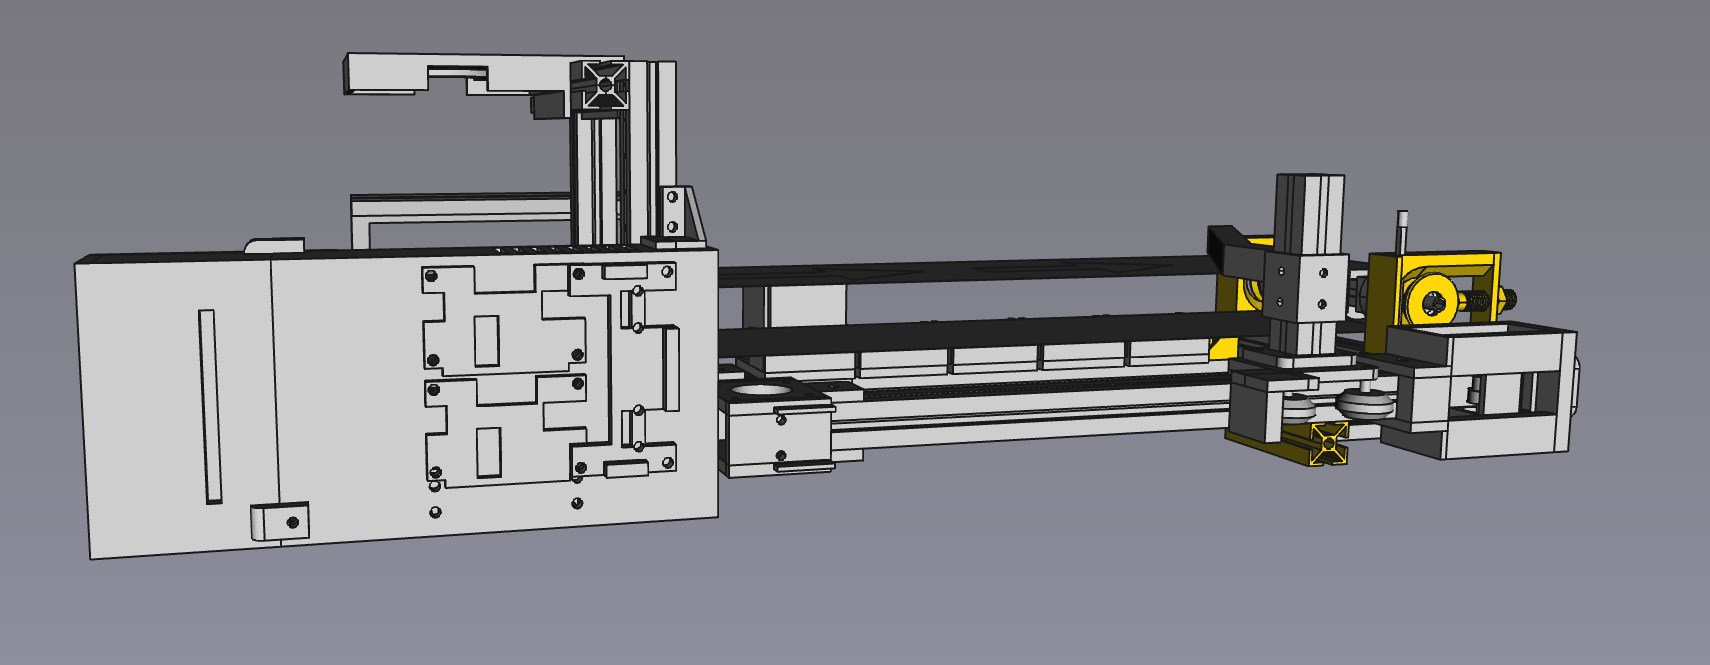
\includegraphics[height=8cm]{imgs/freecad/wholeback.jpg}
        \caption{Back View of the Mechanical Design}
    \end{minipage}
\end{figure}

From the back view of the system, the PSU enclosure is clearly visible with mounting plates for the step-down converters. A belt-driven arm is visible on the back, making use of another NEMA17 motor to drive it and a belt tensioner to ensure the belt is taut. The belt-driven arm is used to push components off the conveyor belt into the sorting bins. The tensioners for the conveyor belt itself are also visible in the back view on the right side.

\subsubsection{Power Supply Unit Enclosure}
\label{sec:power-supply-unit-enclosure}

Due to the potential of high-current carrying wires, the PSU has been enclosed in a 3D printed case, which prevents accidental contact with the PSU's terminals.

\begin{figure}[H]
    \begin{minipage}[h]{0.95\textwidth}
        \centering
        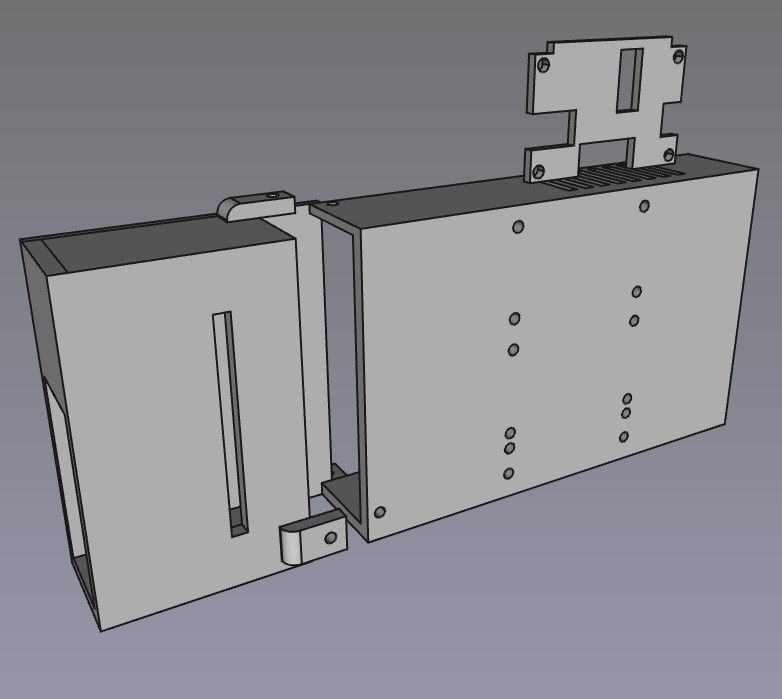
\includegraphics[height=8cm]{imgs/freecad/psu_mount.jpg}
        \caption{PSU Enclosure}
    \end{minipage}
\end{figure}

The PSU enclosure contains several components;
\begin{mylist}
    \item PSU Container: The PSU container is designed to house the 24V 6.25A power supply unit, and provides mounting holes for the other components. It attaches to the PSU using M3 screws.
    \item Step-Down Converter Mounts: The step-down converters are mounted on the PSU container using M3 screws. The step-down converters are used to convert the 24V output from the PSU to 12V and 5V for the system, shown by the two mounts at the top of the PSU container.
    \item USB Breakout Mount: For the 12V and 5V power outputs, a USB breakout board is used to provide power to the components, allowing standard cables to be used for power distribution. The USB breakout board is mounted on the right side of the PSU container, connecting to the step-down converters.
    \item PSU Switch Housing: For safety reasons, the connections between the switch and the PSU are enclosed in a housing to prevent accidental contact with the high voltage connections. There is a slot in the Switch Housing for the power cable to pass through to the step-down converters, and a switch snap-fit mount to hold the switch in place on the side.
    \item PSU Mount: The PSU mount is used to mount the PSU container to the 2020 extrusion frame of the system. The mount is screwed into the top of the PSU container and the 2020 extrusion frame, using M3 screws and T-nuts.
\end{mylist}

\begin{figure}[H]
    \hfill
    \begin{minipage}[h]{0.45\textwidth}
        \centering
        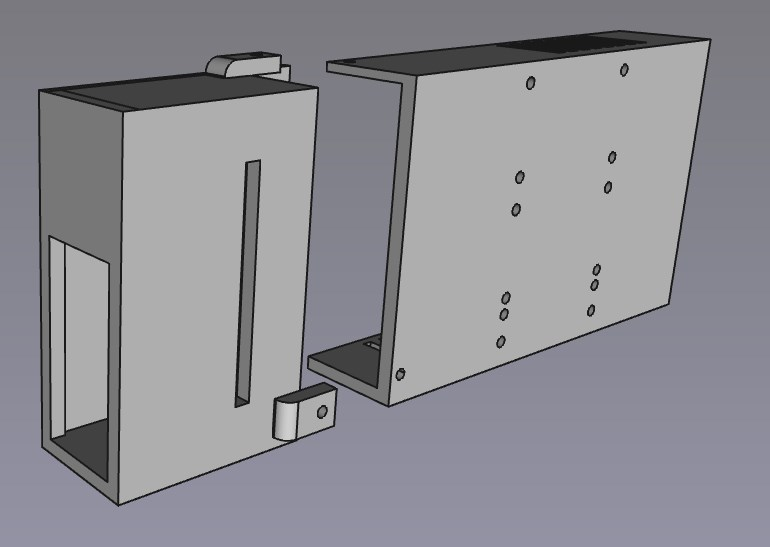
\includegraphics[height=6cm]{imgs/freecad/psu_switch.jpg}
        \caption{PSU Switch Housing}
    \end{minipage}
    \hfill
    \begin{minipage}[h]{0.45\textwidth}
        \centering
        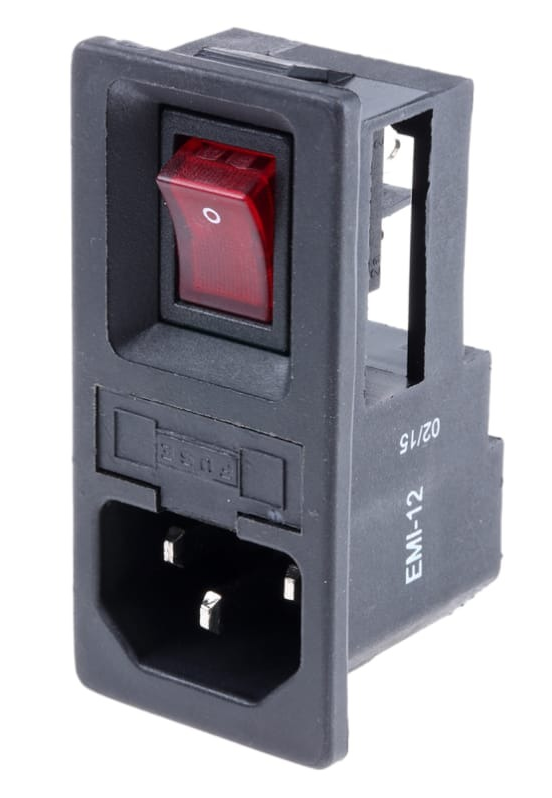
\includegraphics[height=6cm]{imgs/parts/iec_c14.jpg}
        \caption{IEC C14 Power Socket \cite{rsproc14switch}}
        \end{minipage}
    \hfill
\end{figure}

A standard IEC C14 power connector and an RS Pro Snap-In Fused Rocker Switch \cite{rsproc14switch} are used to connect the PSU to the mains power. As the power supply is a 6.25A power supply, a 6A fuse was chosen for the switch, which is the closest available fuse rating to the power supply's current rating. This ensures that the fuse will trigger before the power supply is damaged, should there be a short circuit in the system. For wiring the power supply and connecting the step-down converters, 18AWG wire was chosen which is rated for 17A \cite{18awgwire}, which is sufficient for the system's power consumption. The wire is securely crimped to the power supply using a crimping tool.

\begin{minipage}{0.5\textwidth}
    \centering
    {\fontsize{8pt}{11pt}\selectfont
    \begin{tabularx}{\textwidth}{|X|p{1cm}|p{1cm}|X|}
        \hline
        \textbf{Test} & \textbf{Result} & \textbf{Req} & \textbf{Description} \\ \hline
        Earth Continuity & 0.06$\Omega$ & $\leq$ 0.1$\Omega$ & Verifies the earth wire is connected. \\ \hline
        Earth Leakage & 0.2mA & $\leq$ 0.75mA & Ensure the touchable metal parts cannot cause harm. \\ \hline
        Insulation Resistance & 320M$\Omega$ & $\geq$ 1M$\Omega$ & Ensure wires are sufficiently insulated. \\ \hline
    \end{tabularx}
    }
    \captionof{table}{PAT Testing Results}
    \label{tab:pat}
\end{minipage}%
\hfill % Adds horizontal space between the table and the image
\begin{minipage}{0.45\textwidth}
    \centering
    \raisebox{-\height}{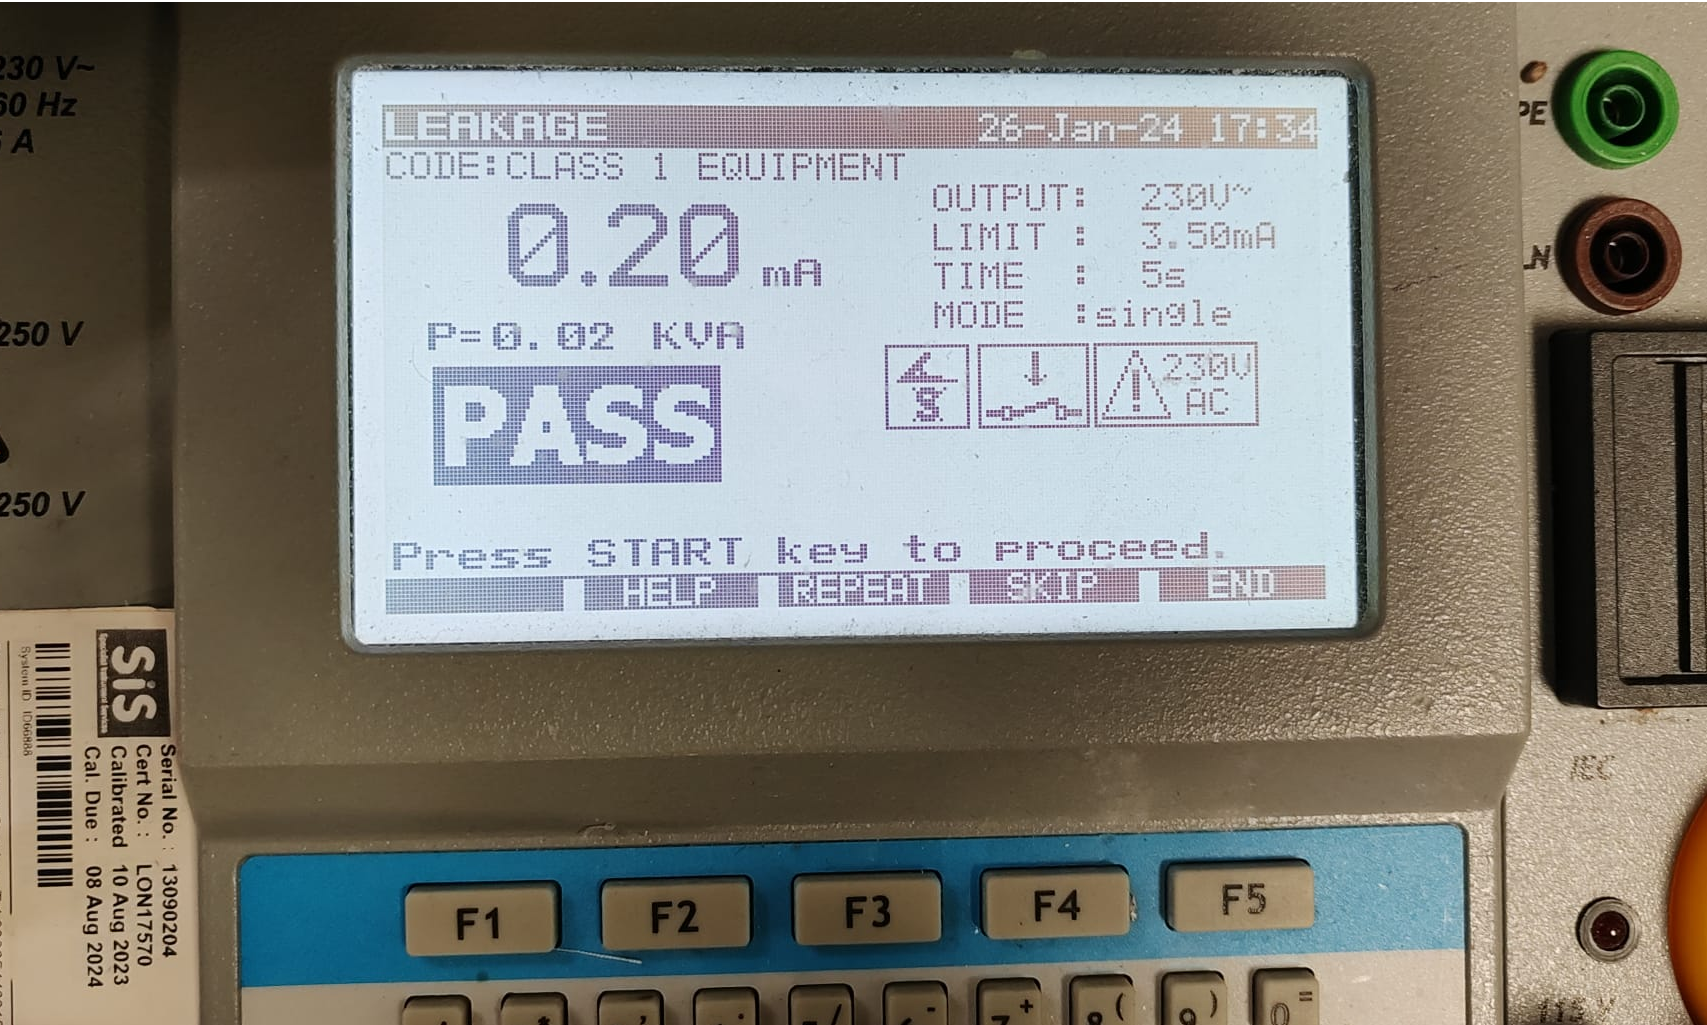
\includegraphics[height=3.5cm]{imgs/pattesting.jpeg}}
    \captionof{figure}{PAT Testing Machine}
    \label{fig:pat}
\end{minipage}


Due to the concern of electrical safety,  the power supply has been PAT tested by technicians in the Level 1 Labs and has been deemed safe for use. PAT (Portable Appliance Testing) is a process by which electrical appliances are routinely checked for safety \cite{patwiki, patspec}. The results of the PAT test are shown in \autoref{tab:pat}.

\begin{figure}[H]
    \begin{minipage}[h]{0.95\textwidth}
        \centering
        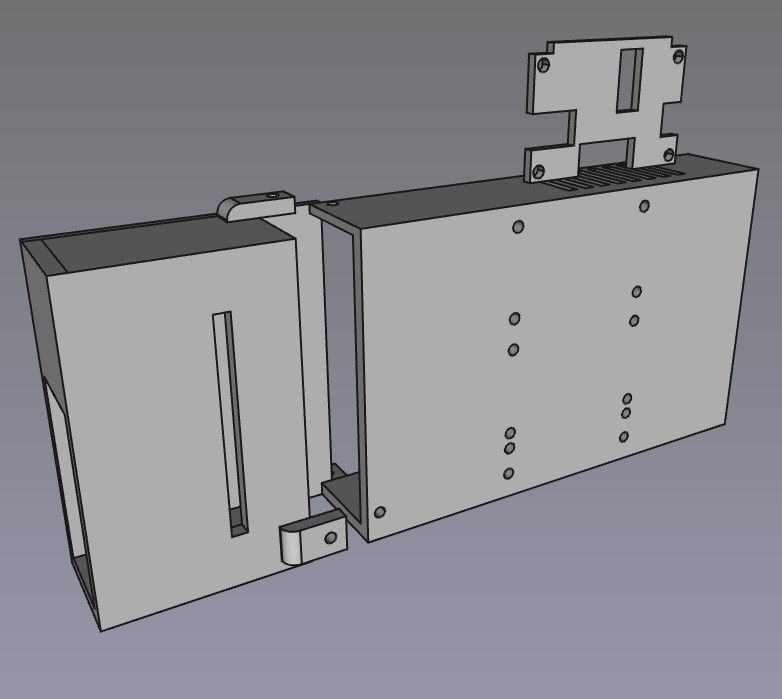
\includegraphics[height=8cm]{imgs/freecad/psu_mount.jpg}
        \caption{Final PSU Enclosure}
        \label{fig:psuenclosure}
    \end{minipage}
\end{figure}
\todo{show actual PSU}

As shown in \autoref{fig:psuenclosure}, the final PSU enclosure is shown to be working with the 5V and 12V outputs connected to the mounted USB breakout boards.

\subsubsection{LCD Mount}
\label{sec:lcd-mount}
For the DFRobot 7" LCD, a mount was designed to hold the LCD in place on the front of the system. The LCD is affixed at a 15$^{\circ}$ angle to the front of the system, allowing for easy viewing by the user. The mount is designed to be attached to the 2020 extrusion frame of the system, using M3 screws and T-nuts.

\begin{figure}[ht]
    \centering
    \begin{minipage}{0.45\textwidth}
        \centering
        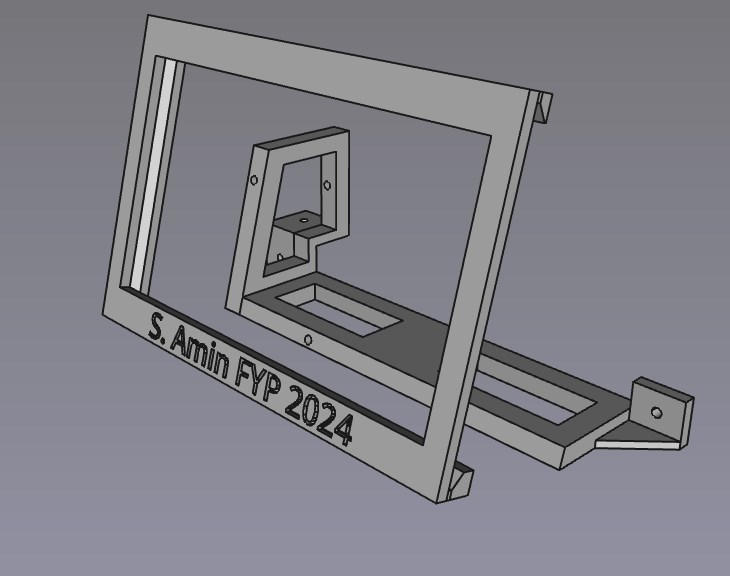
\includegraphics[height=6cm]{imgs/freecad/lcd_mount2.jpg}
        \caption{LCD Mount}
    \end{minipage}\hfill
    \begin{minipage}{0.45\textwidth}
        \centering
        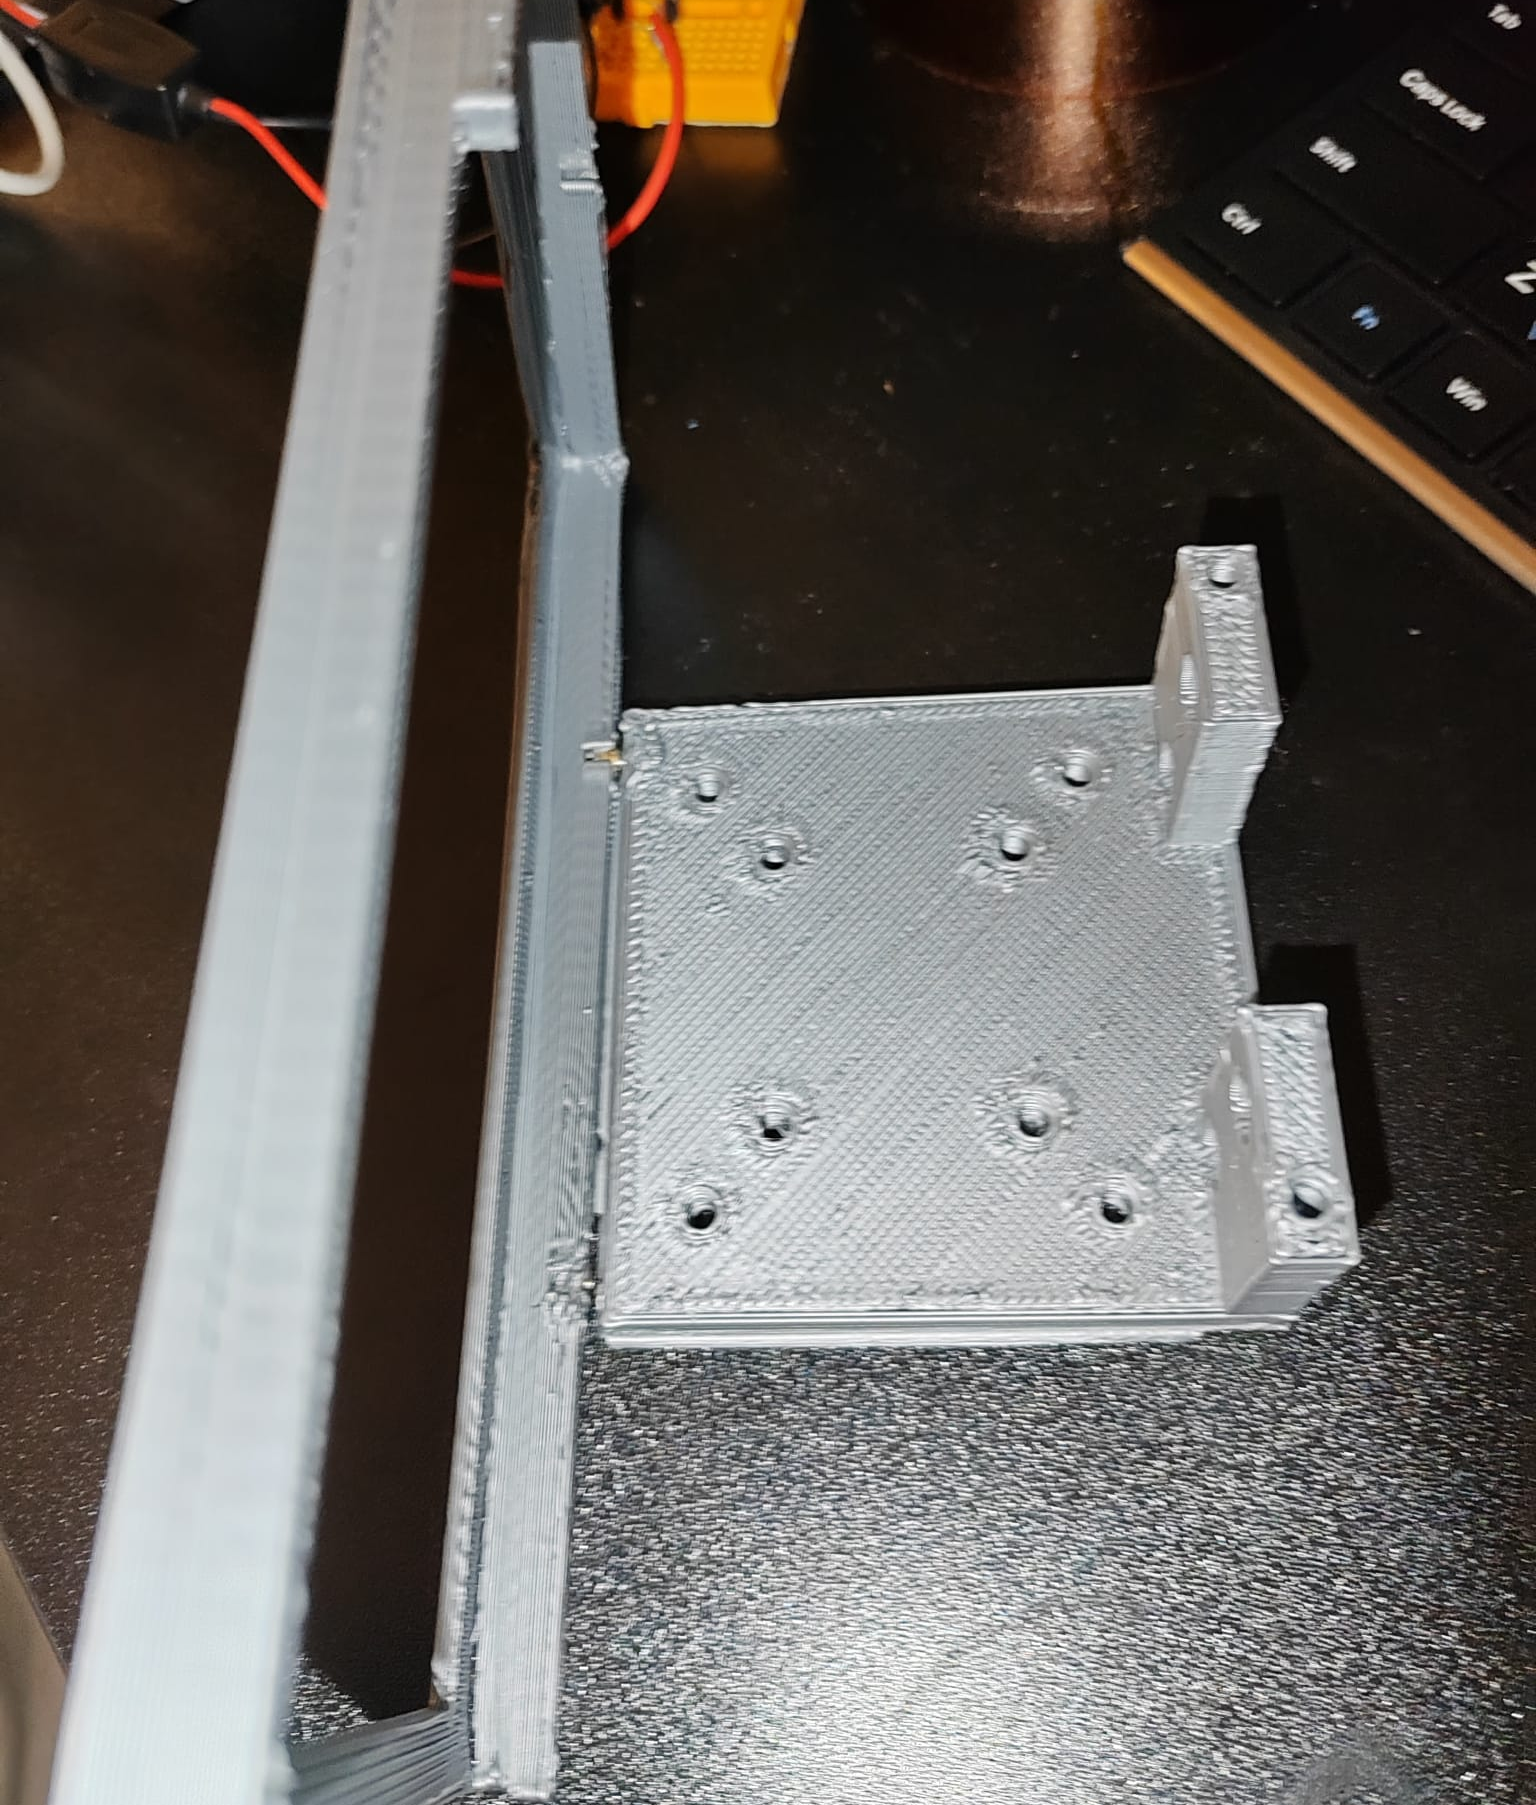
\includegraphics[height=6cm]{imgs/design/unbracedscreen.jpeg}
        \caption{Unbraced LCD Mount}
        \label{fig:brokenlcd}
    \end{minipage}
\end{figure}

The design consists of two parts;
\begin{mylist}
    \item LCD Cover: The LCD cover is designed to hold the LCD in place. It contains a small gap that the LCD fits into, preventing it from falling out with the help of friction.
    \item LCD Extrusion Mount: The LCD extrusion mount is designed to be attached to the 2020 extrusion frame of the system. It contains screw holes for the LCD Cover to be attached to, and screw holes for the 2020 extrusion frame. It also contains a support for the LCD cover to rest on, preventing it from breaking off, as it did in previous iterations, as shown in \autoref{fig:brokenlcd}.
\end{mylist}

\subsubsection{Conveyor Belt}
\label{sec:conveyor-belt}
The conveyor belt is a key component of the system, as it is used to transport components from the input side to the bins. As such, it is the largest component of the system, and so makes use of 2020 aluminium extrusion as its skeleton. The conveyor belt has two rollers; one actively driven by a NEMA17 stepper motor, and the other is a free roller. The conveyor belt relies on friction to turn the idle roller, so it is essential that the belt is taut. To ensure this, belt tensioners are used on the idler side of the conveyor belt.

\begin{figure}[H]
    \begin{minipage}[h]{0.95\textwidth}
        \centering
        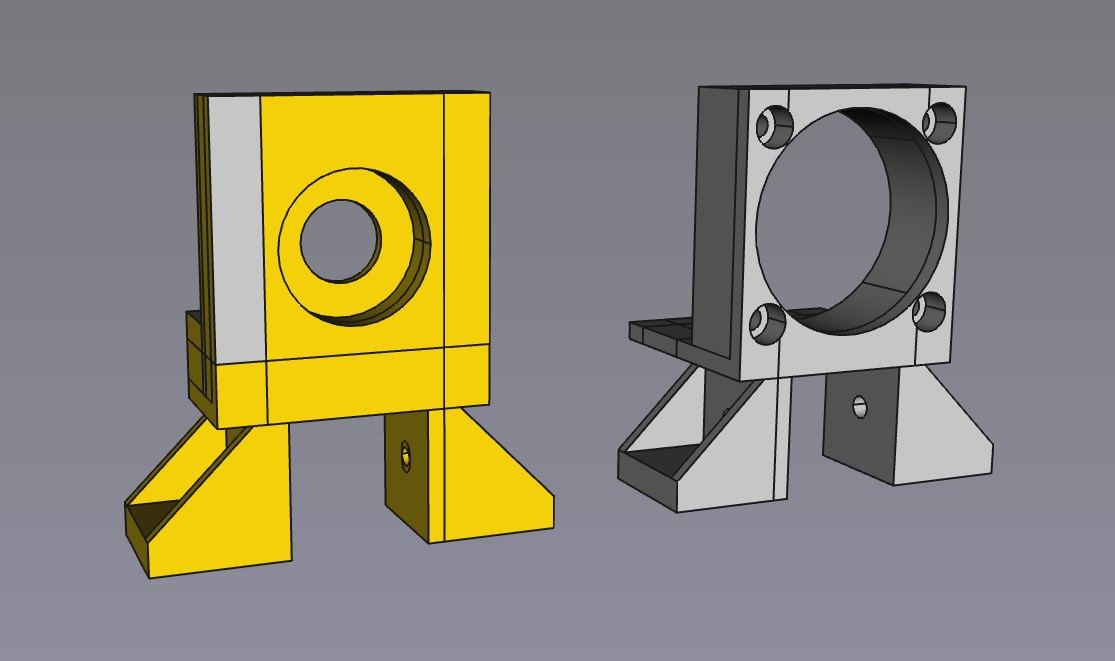
\includegraphics[height=8cm]{imgs/freecad/conveyor_driven.jpg}
        \caption{Driven Conveyor Roller}
        \label{fig:conveyordriven}
    \end{minipage}
\end{figure}

\autoref{fig:conveyordriven} shows the mounts for the driven conveyor roller, the right side mounting the NEMA17 stepper through four M3 screws, and the left side mounting the other side of the roller by allowing it to rotate freely in the mount. The left side contains a space for a 608ZZ bearing to be inserted, which allows the roller to rotate freely without friction (8x22x7mm). 

\begin{figure}[H]
    \begin{minipage}[h]{0.95\textwidth}
        \centering
        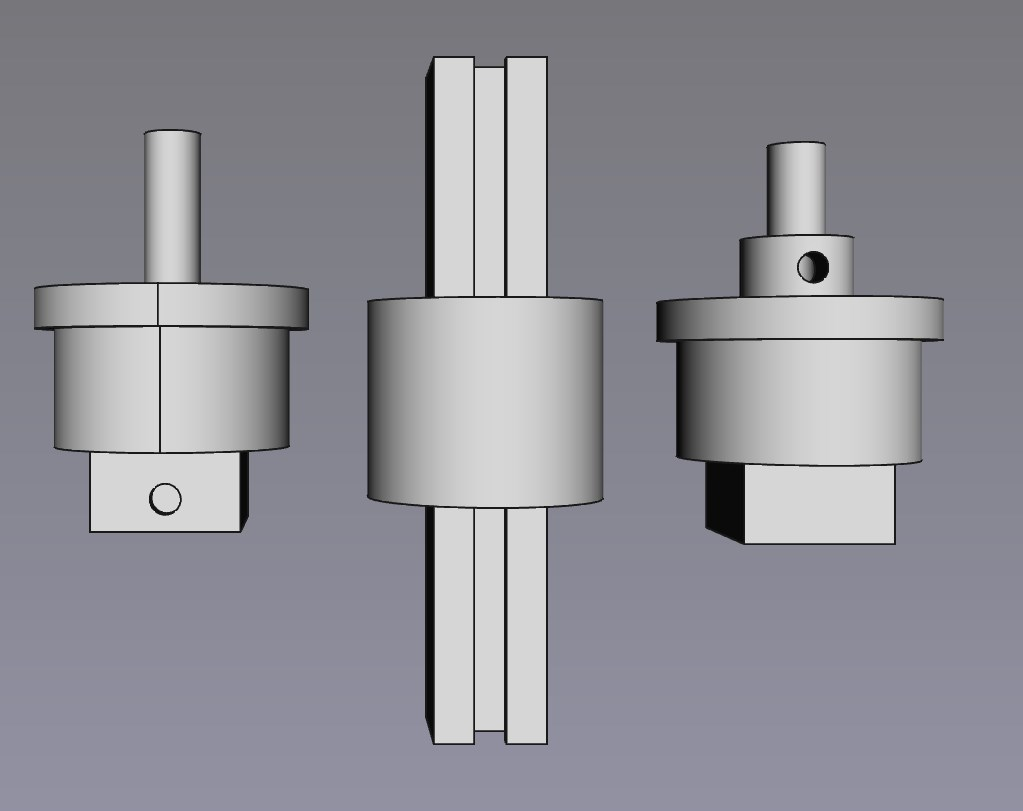
\includegraphics[height=8cm]{imgs/freecad/rollers.jpg}
        \caption{Conveyor Belt Rollers}
        \label{fig:conveyorrollers}
    \end{minipage}
\end{figure}

\autoref{fig:conveyorrollers} shows the rollers themselves, with non-driven end rollers on the left, the adjustable-length roller body in the middle, and the motor-coupled roller on the right. During initial development, it was unsure what the width of the conveyor belt would be, so a design was made to allow for the length of the rollers to be adjusted. This is done by using a screw on the roller ends to adjust where it locks onto the roller body, enabling the length of the roller to be adjusted. The roller is coupled to the motor by screwing an M3 screw into the side of the roller which pushes against the motor shaft, allowing the motor to drive the roller. \autoref{fig:adjustablerollers} shows the adjustable roller design.

\begin{figure}[H]
    \begin{minipage}[h]{0.95\textwidth}
        \centering
        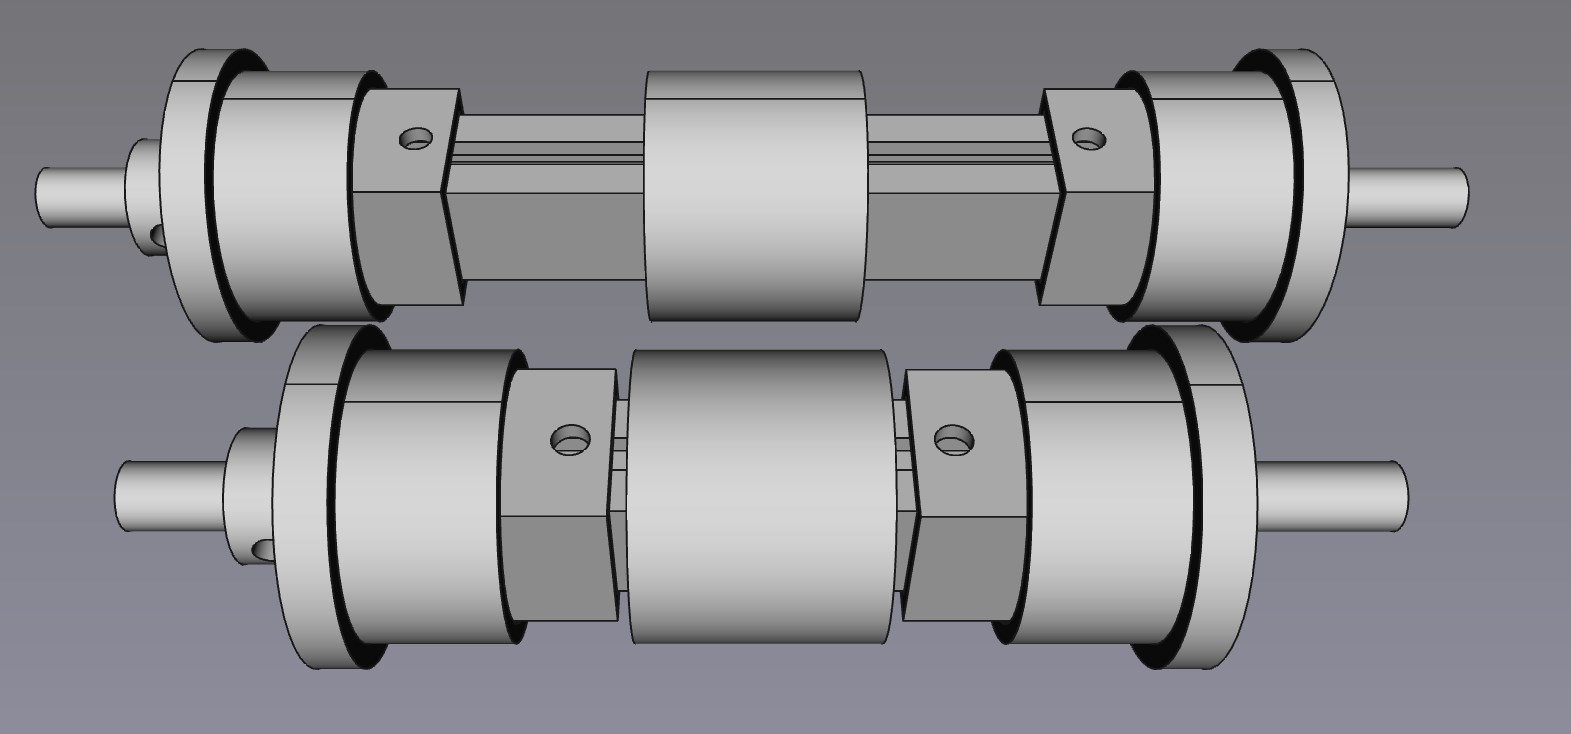
\includegraphics[height=7cm]{imgs/freecad/adjustablerollers.jpg}
        \caption{Adjustable Conveyor Rollers}
        \label{fig:adjustablerollers}
    \end{minipage}
\end{figure}

The 